\documentclass[sigconf,anonymous]{acmart}

% Personal provisional manuscript. This file is not the authoritative LOCUS
% manuscript and is intentionally excluded from project planning and claims.
\let\Bbbk\relax
\usepackage{amsmath,amssymb,amsfonts}
\usepackage{graphicx}
\usepackage{textcomp}
\usepackage{xcolor}
\usepackage{booktabs}
\usepackage{array}
\usepackage{url}
\usepackage{hyperref}
\usepackage{tikz}
\usetikzlibrary{arrows.meta,positioning,fit}
\setlength{\emergencystretch}{2em}

\def\BibTeX{{\rm B\kern-.05em{\sc i\kern-.025em b}\kern-.08em
    T\kern-.1667em\lower.7ex\hbox{E}\kern-.125emX}}

\newcommand{\LOCUS}{\textsf{LOCUS}}
\newcommand{\Yi}{\ensuremath{\mathsf{Yi}}}
\newcommand{\APPSS}{\ensuremath{\mathsf{aPPSS}}}
\newcommand{\CuePolicy}{\ensuremath{\mathsf{CuePolicy}}}
\newcommand{\Encode}{\ensuremath{\mathsf{Encode}}}
\newcommand{\Hash}{\ensuremath{\mathsf{H}}}
\newcommand{\HKDF}{\ensuremath{\mathsf{HKDF}}}
\newcommand{\AEAD}{\ensuremath{\mathsf{AEAD}}}
\newcommand{\Setup}{\ensuremath{\mathsf{Setup}}}
\newcommand{\Recover}{\ensuremath{\mathsf{Recover}}}
\newcommand{\TBD}{\textbf{TBD}}

\acmYear{2027}
\copyrightyear{2027}
\setcopyright{acmlicensed}
\acmConference[ASIACCS '27]{Proceedings of the 22nd ACM Asia Conference on Computer and Communications Security}{July 12--16, 2027}{Macau, China}
\acmBooktitle{Proceedings of the 22nd ACM Asia Conference on Computer and Communications Security (ASIACCS '27), July 12--16, 2027, Macau, China}
\acmDOI{10.1145/XXXXXXX.XXXXXXX}
\acmISBN{979-8-XXXX-XXXX-X/27/07}

\begin{document}

\title{LOCUS: Integrated Storage-Separated Private-Key Recovery with Selectable Threshold Suites}
\renewcommand{\shortauthors}{anonymous}

\begin{abstract}
Long-lived private keys create a recovery dilemma: a mechanism must remain
usable after device loss, yet a leaked backup must not become a local oracle
for testing predictable human input. \LOCUS\ is an integrated recovery system
that composes deterministic, versioned processing of structured recovery input
with an explicitly selected threshold recovery suite and storage-separated
authenticated encryption. The active client alone converts structured input
through a \CuePolicy, derives suite-bound password material, obtains a
high-entropy recovery secret through either the Yi threshold
password-authenticated secret-sharing suite or an augmented
password-protected secret-sharing (\APPSS) suite, and derives an AES-256-GCM
wrapping key. The cloud role stores only the encrypted private-key backup and
public authenticated configuration; five separately identified authorizers
hold suite-specific state, with paired 2-of-3 and 3-of-5 reconstruction
profiles and a distinct 4-of-5 authorization quorum.

The reference implementation connects a loopback Manager, a narrowly scoped
container controller, dynamically created clean Client interfaces,
authenticated admission and discovery, a storage gateway and local
S3-compatible provider, a resolver, and five party services. A signed
descriptor and live party summaries bind one suite, policy, membership, and
epoch without recovery-time fallback. Aggregate retained experiments exercise
42 persistent-state scenarios and 30 payload-free application-flow scenarios
over the managed graph. A separately versioned performance methodology
specifies 324 scheduled observations across four matched suite/topology arms;
its numerical results remain provisional in this personal draft. The resulting
claim is deliberately narrow: cloud-only, below-threshold party, and matching
cloud-plus-below-threshold persistent states do not expose a local offline
cue-testing predicate under the inherited suite assumptions. \LOCUS\ does not
claim new threshold cryptography, cue memorability, global rollback-resistant
attempt control, independent administration, or production readiness.
\end{abstract}

\ccsdesc[500]{Security and privacy~Key management}
\ccsdesc[500]{Security and privacy~Security protocols}
\ccsdesc[300]{Security and privacy~Distributed systems security}

\keywords{private-key recovery, threshold password-authenticated secret
sharing, password-protected secret sharing, cloud backup, clean-client
recovery, storage separation}

\maketitle

\begin{center}
\fcolorbox{red!70!black}{red!5}{%
\parbox{0.94\linewidth}{\footnotesize
\textbf{Personal provisional status draft.}
This document is not the authoritative LOCUS manuscript, does not modify the
project plan or claim matrix, and is not a source of evidence. It presents the
intended completed-system narrative so that the project can be reviewed as a
whole. Retained P8 evidence is reported only at its established scope.
Unavailable P9 measurements, independent-review outcomes, and final artifact
digests are marked \TBD\ rather than invented.}}
\end{center}

\section{Introduction}
\label{sec:introduction}

Private keys protect encrypted archives, end-to-end encrypted accounts,
identities, credentials, and self-custodied assets. Their security depends on
exclusive control, but that same exclusivity makes loss catastrophic. Recovery
systems generally relax one of three properties. Custodial systems concentrate
recovery power in one operator. High-entropy recovery codes preserve
cryptographic strength but create another long-lived object that must be kept
available. Password-encrypted backups remain convenient but can become
offline-guessing targets when ciphertext and a password verifier are copied.
Social and threshold recovery distribute authority, but often leave the
human-input, discovery, encrypted-storage, and replacement-device workflows
outside the evaluated protocol.

\LOCUS\ studies a different systems composition. A client deterministically
converts structured recovery input into exact bytes. Those bytes are not used
directly as an encryption key and are not stored as a verifier. Instead, they
mediate an online threshold protocol that yields high-entropy recovery
material. The client derives an authenticated-encryption key from that
material, while an object-storage role keeps only the encrypted private-key
backup and public authenticated configuration. The intended persistent-state
boundary is therefore:
\[
  \text{cloud} \;\perp\; \text{threshold state} \;\perp\;
  \text{complete client secret path}.
\]
The design is useful only if the full replacement-device path preserves this
boundary. It must authenticate discovery, descriptors, party identities,
admission, storage operations, and lifecycle transitions without reintroducing
a cue-derived predicate.

Structured input is not automatically memorable or unpredictable. Studies of
personal-knowledge questions, graphical cues, and location-based fallback
authentication show both the attraction and the hazards of such
interfaces~\cite{Bonneau2015Secrets,Biddle2012Graphical,AlAmeen2017GeoPass,Hang2015LocationFallback}.
\LOCUS\ therefore separates two questions. A \CuePolicy\ is an engineering
contract for deterministic bytes, ambiguity, duplicates, resolver behavior,
and versioning. Whether people can reliably remember or safely select inputs
for a particular policy is an empirical usability question that this work does
not answer.

The current system supports two independently selected inherited recovery
suites. The frozen Yi TPASS suite follows Yi et
al.~\cite{Yi2015TPASS,Yi2019TPASS}. The second suite instantiates the
Figure-4 augmented password-protected secret-sharing construction of
Dziembowski et al.'s \emph{Password-Protected Threshold Signatures}, using an
RFC 9497 ristretto255/SHA-512 OPRF~\cite{RFC9497OPRF}. The suites are not
interchangeable at recovery time and have different threshold-compromise
semantics. Threshold Yi state directly exposes its high-entropy recovered
secret. Threshold \APPSS\ state and public state enable unrate-limited
dictionary testing, with the correct candidate yielding the recovery secret.
Below reconstruction threshold, both are intended to require participation by
an uncompromised online party to evaluate a candidate.

\paragraph{Contributions.}
This provisional manuscript organizes the project around four contributions:

\begin{enumerate}
  \item a versioned \CuePolicy\ boundary that converts structured input into
  deterministic client-local bytes without persisting a cue verifier;
  \item a suite-neutral recovery composition that binds exactly one Yi or
  \APPSS\ suite to each epoch, keeps reconstruction threshold separate from
  authorization quorum, and feeds the recovered high-entropy value into a
  common HKDF/AES-256-GCM backup path;
  \item an integrated managed reference system spanning clean Clients,
  authenticated discovery and admission, descriptor/current-state checks,
  storage gateway/provider, resolver, and five party processes; and
  \item a claim-scoped evaluation methodology that binds state, flow,
  performance, failure, and artifact observations to the exact managed
  deployment without pooling historical or component evidence.
\end{enumerate}

\paragraph{Scope.}
\LOCUS\ claims no new TPASS, PPSS, \APPSS, OPRF, secret-sharing, or
authenticated-encryption construction. The system tests whether explicit
interfaces and service boundaries preserve the security meaning inherited
from those constructions. It does not establish human memorability,
production-hardening, side-channel resistance, independently administered
parties, or a lifetime/global online-attempt limit.

\section{Goals, System Model, and Threat Model}
\label{sec:model}

\subsection{Security Goal}

Let \(M\) be structured recovery input and let an approved policy version
produce \(Z_M=\CuePolicy_v(M)\) or fail. Let \(p_M\) be suite-bound password
material, \(S_R\) the high-entropy recovery output, and \(B\) the encrypted
backup. The central system goal is:

\begin{quote}
Cloud-only, fewer-than-reconstruction-threshold party, and matching
cloud-plus-below-threshold persistent states do not expose a local offline
predicate for testing a candidate \(M'\). Candidate evaluation requires
online participation from sufficient authenticated threshold parties, under
the selected suite's assumptions.
\end{quote}

This is a statement about specified persistent views, not about the entropy of
\(M\), compromise of an active client, timing leakage, or the consequences of
reaching the reconstruction threshold.

\subsection{Entities and Trust Boundaries}

\begin{table*}[t]
\centering
\caption{Roles in the managed reference system.}
\label{tab:roles}
\footnotesize
\begin{tabular}{p{0.15\linewidth}p{0.31\linewidth}p{0.45\linewidth}}
\toprule
\textbf{Role} & \textbf{Responsibility} & \textbf{Security boundary} \\
\midrule
User/browser & Supplies synthetic structured input and invokes enrollment or
recovery through loopback pages & Browser and active managed Client jointly
form the transient secret boundary; browser history, OS capture, and already
loaded pages are not erased by container reset \\
\addlinespace
Manager & Starts the common system and requests creation, stop, restart,
kill/start, or destruction of managed Clients & Never receives cues, package
bytes, suite state, recovered secrets, wrapping keys, or plaintext protected
keys; has no Docker socket \\
\addlinespace
Controller & Executes a fixed allowlisted set of lifecycle operations on exact
project-labeled Client containers & Holds the root-equivalent Docker socket and
is trusted operator infrastructure; accepts no caller-supplied image, command,
mount, host path, network, or arbitrary identifier \\
\addlinespace
Managed Client & Runs the thin UI and client state machines, performs policy
processing, suite operations, backup encryption/decryption, and package
validation & Only active Client may transiently handle the complete secret
path; no protocol state is shared between Client instances \\
\addlinespace
Operator/discovery & Signs descriptors and current pointers and returns public
configuration & Operator signing is not a self-authenticating trust root;
Clients begin with installed trust and verify live party summaries \\
\addlinespace
Admission & Issues short-lived, proof-key-bound capabilities for exact
operations & Independent of cues and suite correctness; admission availability
is a recovery prerequisite, not a hidden recovery factor \\
\addlinespace
Storage gateway/provider & Maps admitted operations to immutable backups,
descriptors, bundles, and a mutable current pointer & Provider credentials
remain gateway-side; Clients cannot list a bucket or receive storage
credentials \\
\addlinespace
Resolver & Implements the policy-specific resolution contract when required &
May learn lookup input; local hashing after lookup does not hide it \\
\addlinespace
Five parties & Every party authorizes; the selected subset also holds Yi or
\APPSS\ state & Reconstruction is 2-of-3 or 3-of-5, while authorization is
separately typed as 4-of-5 \\
\bottomrule
\end{tabular}
\end{table*}

Figure~\ref{fig:architecture} summarizes the deployed same-host graph.
Only Manager and Client pages are published on host loopback. The Manager and
controller share the internal \emph{management} network. The controller and
managed Clients share the disjoint \emph{client-lifecycle} network. Separate
\emph{manager-edge} and \emph{browser-edge} networks publish the Manager and
Client pages and do not create a container-level Manager-to-Client route.
Managed Clients reach the protocol service plane, but neither browser
interface contacts the provider, resolver, admission service, parties, or
Docker engine directly.

\begin{figure*}[t]
\centering
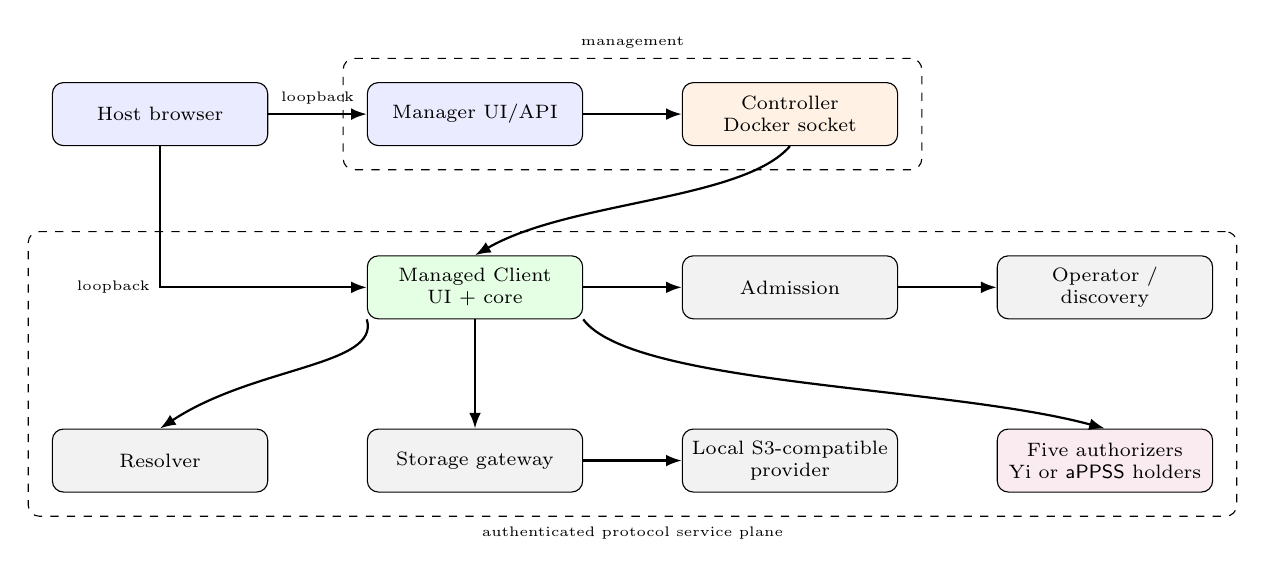
\begin{tikzpicture}[
  box/.style={draw,rounded corners,align=center,font=\scriptsize,
              minimum height=8mm,text width=25mm},
  trust/.style={draw,dashed,rounded corners,inner sep=3mm},
  arr/.style={-{Latex[length=2mm]},thick}
]
\node[box,fill=blue!8] (browser) at (0,2.2) {Host browser};
\node[box,fill=blue!8] (manager) at (4,2.2) {Manager UI/API};
\node[box,fill=orange!10] (controller) at (8,2.2) {Controller\\Docker socket};
\node[box,fill=green!10] (client) at (4,0) {Managed Client\\UI + core};
\node[box,fill=gray!10] (admission) at (8,0) {Admission};
\node[box,fill=gray!10] (operator) at (12,0) {Operator /\\discovery};
\node[box,fill=gray!10] (resolver) at (0,-2.2) {Resolver};
\node[box,fill=gray!10] (gateway) at (4,-2.2) {Storage gateway};
\node[box,fill=gray!10] (provider) at (8,-2.2) {Local S3-compatible\\provider};
\node[box,fill=purple!8] (parties) at (12,-2.2)
  {Five authorizers\\Yi or \APPSS\ holders};

\draw[arr] (browser) -- node[above,font=\tiny]{loopback} (manager);
\draw[arr] (browser) |- node[left,font=\tiny]{loopback} (client);
\draw[arr] (manager) -- (controller);
\draw[arr] (controller.south) .. controls (7.4,1.1) and (5.2,1.1) ..
  (client.north);
\draw[arr] (client) -- (admission);
\draw[arr] (admission) -- (operator);
\draw[arr] (client) -- (gateway);
\draw[arr] (gateway) -- (provider);
\draw[arr] (client.south west) .. controls (2.8,-1.0) and (1.2,-1.0) ..
  (resolver.north);
\draw[arr] (client.south east) .. controls (6.0,-1.25) and (10.0,-1.25) ..
  (parties.north);
\node[trust,fit=(manager)(controller),label={[font=\tiny]above:management}] {};
\node[trust,fit=(client)(admission)(operator)(resolver)(gateway)(provider)(parties),
      label={[font=\tiny]below:authenticated protocol service plane}] {};
\end{tikzpicture}
\caption{Managed integrated reference system. Network boxes are conceptual:
all roles execute on one Docker engine under one operator. This demonstrates
process, credential, and network separation, not host separation or
independent administration.}
\Description{A host browser reaches a loopback Manager and a separate managed
Client. The Manager reaches only the container controller. The Client reaches
admission, operator and discovery, storage gateway and provider, resolver, and
five authorizers. Dashed boxes distinguish management from the authenticated
protocol service plane.}
\label{fig:architecture}
\end{figure*}

\subsection{Adversary Classes}

\paragraph{Cloud/public-state adversary.}
The adversary obtains the encrypted backup, signed descriptor, bundle,
manifest, and current-pointer state. It may delete, replay, or substitute
objects. Integrity and cross-binding checks can detect malformed or
inconsistent state, but availability is not guaranteed.

\paragraph{Below-threshold holder adversary.}
The adversary obtains static, read-only persistent state from fewer than \(k\)
matching suite holders, possibly together with the cloud view. The claim
excludes live compromise that can make an honest party evaluate arbitrary
queries, side channels, volatile memory, and secret-bearing crash artifacts.

\paragraph{Threshold holder adversary.}
The adversary obtains at least \(k\) matching holder states. This is outside
the main below-threshold claim. Its consequence is suite-specific: Yi exposes
the shared high-entropy recovery value directly, whereas \APPSS\ exposes an
offline dictionary predicate and yields the recovery value for a correct
candidate.

\paragraph{Online adversary.}
The adversary submits candidates through admitted recovery sessions. Signed
local party records provide diagnostic evidence, and authorization requires
four of five authorizers, but no monotonic global authority survives
coordinated rollback. Accordingly, \LOCUS\ makes no global or lifetime attempt
bound.

\paragraph{Control-plane adversary.}
The controller and Docker socket are root-equivalent trusted infrastructure.
Compromise can subvert containers and therefore defeats process isolation.
The Manager is less privileged but remains an availability and lifecycle
control point.

\paragraph{Provider, resolver, and metadata observers.}
These roles may correlate a pseudonymous subject, backup identifier, epoch,
policy and suite identifiers, memberships, object sizes, access times, and
endpoints. A resolver may observe a selected query. The system aims to exclude
raw cues and secret-derived verifiers from persistent state, not to provide
traffic-analysis anonymity.

\subsection{Assumptions}

The installed application supplies authentic operator and party roots. TLS
and signature algorithms operate as specified. HKDF-SHA-256 and AES-256-GCM
provide their standard properties~\cite{HKDF2010,RFC5116AEAD}. At least one
required online holder remains uncompromised for the below-threshold claim,
and the active Client is trusted while it processes secrets. Suite-specific
claims inherit the source construction, random-oracle, OPRF, group, and
corruption assumptions; implementation tests are not cryptographic proofs.

\section{Design Requirements and Invariants}
\label{sec:requirements}

\paragraph{Deterministic policy boundary.}
Every policy declares accepted structure, cardinality, resolver behavior,
canonicalization, ambiguity, duplicate, and version rules. It returns exactly
one byte string or fails. It must not emit hints, fuzzy alternatives, or
persisted candidate verifiers.

\paragraph{One suite per epoch.}
Enrollment or successor creation explicitly selects one registered suite and
topology. The authenticated descriptor binds that choice. Recovery derives the
adapter only from verified configuration: no automatic fallback, trial of
another suite, cross-suite share mixing, or in-place conversion is allowed.

\paragraph{Threshold separation.}
The type for suite reconstruction \(k\)-of-\(n\) is distinct from the
authorization quorum. The implemented profiles are Yi and \APPSS\ at 2-of-3
and 3-of-5 over five authorizers, with authorization fixed at 4-of-5.

\paragraph{Protected path.}
The active Client alone executes
\[
\begin{split}
M &\xrightarrow{\CuePolicy_v} Z_M
  \xrightarrow{\text{suite domain}} p_M
  \xrightarrow{\Setup/\Recover} S_R \\
  &\xrightarrow{\HKDF\text{-SHA-256}} K_{\mathrm{wrap}}
  \xrightarrow{\mathrm{AES\mbox{-}256\mbox{-}GCM}} sk .
\end{split}
\]
Raw cues, selected canonical descriptors, \(Z_M\), \(p_M\), \(S_R\),
\(K_{\mathrm{wrap}}\), and plaintext \(sk\) must not persist in cloud, party,
Manager, controller, package, or retained evidence state.

\paragraph{Authenticated bootstrap.}
A descriptor cannot authenticate its own trust root. Installed trust
authenticates the discovery endpoint, operator key, party identities, and
endpoints. A clean Client verifies signed current state and obtains a fresh
4-of-5 matching party-current quorum before cue-dependent work.

\paragraph{Atomic lifecycle.}
A predecessor remains recoverable until successor party state, backup,
descriptor, bundle, and current pointer are durable and the successor has
recovered the same protected key. Retry behavior is idempotent and bound to
exact request/configuration digests.

\paragraph{Evidence isolation.}
Historical component measurements, frozen deployments, unit vectors, and
P6 process profiles remain controls. Principal system evidence must exercise
the exact Manager-created Client graph and bind source state, resolved
configuration, images, identities, networks, provider, suite, topology,
policy, failure schedule, and Client instances.

\section{Architecture}
\label{sec:architecture}

\subsection{CuePolicy and Resolver Registry}

The \CuePolicy\ interface receives structured input plus registered public
parameters and returns canonical bytes \(Z_M\) or a typed failure. The registry
preserves the original exactly-three location--person-pair policy byte for
byte. Additional policies demonstrate interface generality: exactly three
distinct quantized coordinates, canonical E.164 phone numbers, or constrained
canonical email addresses. Direct-input policies use a \emph{NoResolver}
adapter; the composite location--person policy uses deterministic resolution
in the reproducible profile.

Canonicalization is intentionally strict. Ordering is deterministic; duplicate
semantic values, ambiguous records, unsupported versions, out-of-range
coordinates, and resolver drift fail rather than generating candidate lists.
Public policy metadata identifies the rules, but no cue hash or selected
descriptor is retained as a recovery hint.

\subsection{RecoveryDescriptor, Bundle, and Discovery}

The signed \emph{RecoveryDescriptor} binds:
\begin{itemize}
  \item pseudonymous subject, backup identifier, epoch, and recovery identity;
  \item exact encrypted-backup member digest and byte length;
  \item policy identifier, opaque public parameters, and resolver profile;
  \item one suite identifier, public state, typed \(k,n\), and holder mapping;
  \item five authorizer identities/endpoints, 4-of-5 authorization, admission
  profile, audience, and operation namespace; and
  \item configuration digest and predecessor binding.
\end{itemize}
It excludes raw cues, selected record identifiers, cue digests, candidate
hints, \(p_M\), suite secret state, \(S_R\), \(K_{\mathrm{wrap}}\), plaintext
private keys, credentials, and a trust root that originates only in the
descriptor.

Each immutable recovery bundle is a bounded, deterministic ZIP containing
exactly \texttt{backup.json}, \texttt{descriptor.json}, and
\texttt{manifest.json}. A signed current pointer outside the ZIP binds the
active bundle locator, bundle digest and length, descriptor digest, epoch, and
configuration digest. Exact-member, size, compression, path, canonical
encoding, signature, digest, and cross-object validation occurs before
cue-dependent work.

The default discovery profile uses admission to obtain a short-lived
proof-key-bound capability scoped to one pseudonymous subject, backup,
operation, audience, nonce, and expiry. The storage gateway performs an exact
object operation without returning provider credentials or general listing
authority. An optional signed recovery receipt may carry a discovery handle
and initial public anchor, but it contains neither cues nor credentials and is
not a freshness witness.

\subsection{Managed Clients and Recovery Packages}

Normal startup creates the service plane, Manager, and controller but no
Client. The Manager requests a Client through the controller's fixed API. The
controller assigns a public instance identifier and publishes a separate
loopback UI port. Enrollment executes entirely inside that Client/browser
boundary.

An authenticated client recovery package transfers the bounded public
configuration needed by another clean Client. The package is untrusted input:
its digest/signature, current pointer, descriptor, bundle, party identities,
and current-party summaries are all revalidated. The package cannot override
suite, policy, membership, endpoint, threshold, or fallback behavior.

Stop/start, restart, and kill/start are destructive volatile resets. They
retain the public Client instance identifier but rotate the process proof key
and clear server-side key slots, package caches, operations, and sessions.
Destroy removes both container and instance identifier. A later creation
receives a new identifier. These semantics do not erase browser memory or an
already loaded document.

\subsection{Bootstrap and Credential Lifetime}

A networkless one-shot bootstrap creates synthetic service credentials,
public configuration, empty per-role roots, and fixtures. It must not inject
suite state, cues, protected keys, or secret-bearing Client state. The
bootstrap container runs as root with all capabilities dropped except
\texttt{CHOWN} and \texttt{DAC\_READ\_SEARCH}, has no Docker socket, and exits
before unprivileged runtime services start. Its CA is valid for 366 days and
leaf certificates for 365 days; there is no in-place renewal.

Normal Manager stop and emergency integrated cleanup preserve exact-project
volumes. Only an explicit reset-state operation removes all role/provider
volumes and credentials. That operation irreversibly destroys the local trust
domain and the deployment state required by earlier packages.

\section{Protocol Construction}
\label{sec:protocol}

\subsection{Common Inputs and Domain Separation}

For backup identifier \(b\), epoch \(e\), policy \(v\), selected suite
\(\sigma\), topology \((k,n)\), and authenticated membership \(\mathcal{P}\),
the Client validates an immutable public context \(ctx\). It computes
\[
  Z_M=\CuePolicy_v(M)
\]
or terminates before contacting suite holders. Suite-specific framing derives
\[
  p_M = \Hash(\textsf{domain}_{\sigma}\parallel
              \Encode(ctx)\parallel \Encode(Z_M)).
\]
The Yi and \APPSS\ domains and encodings are disjoint. Public configuration
commits to the exact context so state from a different backup, epoch, policy,
suite, topology, or membership cannot be combined.

After successful setup or recovery, the suite yields \(S_R\). The common
backup path derives
\[
  K_{\mathrm{wrap}} =
  \HKDF_{\mathrm{SHA256}}(S_R,\; salt,\; info(ctx))
\]
and encrypts the private key using AES-256-GCM:
\[
  (c,tag)=\AEAD.\mathsf{Enc}(K_{\mathrm{wrap}},nonce,sk,\mathrm{AAD}(ctx)).
\]
The backup object carries the ciphertext, nonce, tag, and public bindings. It
does not carry a cue verifier.

\subsection{Frozen Yi TPASS Suite}

The Yi adapter preserves the frozen Ristretto255 wire formats and equations.
During setup, the active Client samples a high-entropy group secret and
distributes native TPASS state across the selected holders. During recovery,
the candidate \(p'_M\) is mapped through the frozen suite domain, holders
produce authenticated protocol responses, and a valid \(k\)-subset lets the
Client reconstruct the group secret when the candidate is correct.

The important compromise distinction is that matching threshold Yi state
contains shares sufficient to interpolate the password scalar, secret
exponent, and digest. Thus a threshold persistent-state compromise directly
exposes the high-entropy recovery output; it is not described as merely an
offline dictionary attack. Fewer than \(k\) matching states are covered by
the inherited TPASS threshold claim, subject to the concrete mapping and
review assumptions.

\subsection{Augmented PPSS Suite}

The \APPSS\ profile instantiates only Section 3, Figure 4, and Theorem 2 of
\emph{Password-Protected Threshold Signatures}; it excludes the paper's
threshold-signature, aptSIG, BLS, and PFS layers. It uses security parameter
\(\lambda=128\), Shamir sharing over polynomial-basis
\(\mathrm{GF}(2^{128})\), and one independently keyed RFC 9497
ristretto255/SHA-512 OPRF instance per holder.

For holder \(i\), the Client obtains an OPRF value on the framed \(p_M\) and
derives a 16-byte mask \(\rho_i\). Setup samples
\(s\leftarrow\mathrm{GF}(2^{128})\), shares \(s\) with a degree-\((k-1)\)
polynomial to obtain \(s_i\), and stores
\[
  e_i=s_i\oplus\rho_i
\]
as public masked-share material. A domain-separated SHA-256 call over the
context, \(p_M\), complete canonical \(e\), and encoded \(s\) is split into a
16-byte commitment \(C\) and the 16-byte recovery secret \(S_R\). The Client
uses this \(S_R\) directly in the common HKDF path; it does not create or share
an additional unmasked recovery secret.

For recovery, each selected holder evaluates its bound OPRF instance. The
Client unmasks \(k\) shares, interpolates \(s'\), recomputes the hash, and
accepts only if the commitment matches. Wrong input, invalid OPRF output,
reconstruction failure, commitment mismatch, and final backup failure collapse
to a generic secret-dependent rejection when availability can still be
distinguished safely. Because the base profile uses non-verifiable OPRF mode,
a malicious selected server can cause an unattributable abort.

Matching threshold \APPSS\ holder keys plus public \((e,C)\) permit local,
unrate-limited testing of candidates: incorrect candidates fail \(C\), while
the correct candidate yields \(S_R\). Below threshold, candidate testing still
requires an uncompromised holder's online OPRF participation under the
construction assumptions.

\subsection{Enrollment}
\label{sec:enrollment}

Enrollment proceeds as follows:
\begin{enumerate}
  \item The Client obtains admission and validates installed trust, the exact
  party directory, policy, suite, topology, and authorization profile.
  \item The \CuePolicy\ canonicalizes \(M\), and the selected suite creates
  fresh per-epoch state through authenticated provisioning routes.
  \item The suite yields \(S_R\); the Client encrypts the protected key and
  verifies its stable key identity.
  \item The operator produces the signed descriptor; the Client constructs
  and locally revalidates the deterministic bundle.
  \item The storage gateway creates the immutable bundle and installs the
  authenticated current pointer with compare-and-swap semantics.
  \item Required parties attest readiness. The Client exports a bounded
  recovery package only after durable completion.
\end{enumerate}
Every mutating route is request-bound and idempotent. A retry with identical
bytes returns the same public result; a colliding request identifier with
different bytes fails.

\subsection{Clean-Client Recovery}
\label{sec:recovery}

A clean Client begins without enrollment-client state. It receives installed
trust, a fresh proof key, a recovery handle or package, and transient user
input. It then:
\begin{enumerate}
  \item strictly decodes the package and obtains admitted discovery;
  \item authenticates the current pointer, bundle, descriptor, manifest, and
  backup cross-bindings using installed operator trust;
  \item matches descriptor endpoints and keys against installed party trust;
  \item obtains four matching, short-lived party-current summaries and rejects
  mixed or stale epochs before processing cues;
  \item invokes the descriptor-bound \CuePolicy\ and the one descriptor-bound
  recovery suite, with no selector or fallback;
  \item reconstructs \(S_R\), derives \(K_{\mathrm{wrap}}\), authenticates and
  decrypts the backup, and verifies protected-key identity; and
  \item returns the private key only inside the active Client/browser boundary.
\end{enumerate}
Public parsing, authentication, freshness, and availability failures remain
typed. Secret-dependent failures are deliberately coarsened to reduce
candidate feedback.

\subsection{Successor Epochs}

A suite or policy change creates a fresh successor epoch. The durable
coordinator prepares new party state, encrypts a successor backup, signs and
publishes a new descriptor and bundle, recovers the protected key through the
prepared successor, atomically changes the current pointer, activates the
successor, and only then retires the predecessor. Same-suite and cross-suite
transitions are supported, but state is never translated or mixed; a
cross-suite transition is a complete new setup around the recovered protected
key.

\section{Security Analysis}
\label{sec:security}

\subsection{Persistent-State Views}

Table~\ref{tab:views} states the intended result for the principal static
views. The table is not a new proof: rows inherit their suite assumptions and
are supported operationally only at the exact evidence scope.

\begin{table*}[t]
\centering
\caption{Suite-specific persistent-state consequences.}
\label{tab:views}
\footnotesize
\begin{tabular}{p{0.20\linewidth}p{0.31\linewidth}p{0.38\linewidth}}
\toprule
\textbf{Adversary view} & \textbf{Yi consequence} & \textbf{\APPSS\ consequence} \\
\midrule
Cloud/public state only & Encrypted backup and authenticated public
configuration provide no local candidate predicate & Public \((e,C)\),
descriptor, and encrypted backup provide no local candidate predicate without
holder OPRF keys \\
\addlinespace
Fewer than \(k\) matching holder states & No reconstruction and no local
candidate predicate under the inherited Yi threshold assumptions & No local
candidate predicate; testing requires an uncompromised holder's online OPRF
participation under the \APPSS\ assumptions \\
\addlinespace
Cloud plus fewer than \(k\) matching holder states & Storage separation adds
no missing threshold state, so the combined view remains below threshold &
Ciphertext and public commitment add no missing OPRF key; the combined view
remains below threshold \\
\addlinespace
At least \(k\) matching holder states & Direct interpolation exposes the
high-entropy recovery output & Public state plus threshold holder keys enables
unrate-limited offline candidate testing; a correct candidate yields the
recovery output \\
\bottomrule
\end{tabular}
\end{table*}

\subsection{Why Public Metadata Is Not a Cue Verifier}

The descriptor and pointer expose policy/suite names, topology, membership,
endpoints, public state, object lengths, digests, epochs, and pseudonymous
identifiers. Their ordinary SHA-256 digests bind already public canonical
objects. No digest is computed directly over \(M\), selected resolver records,
\(Z_M\), \(p_M\), \(S_R\), or \(K_{\mathrm{wrap}}\). Consequently, copying the
cloud view does not by itself supply a function that distinguishes a candidate
without the suite interaction. This argument assumes correct domain
separation, canonical decoding, and absence of secret-bearing logs or crash
artifacts.

\subsection{Descriptor Authenticity and Rollback}

A valid signature proves issuance, not freshness. The clean Client begins from
installed trust, authenticates the operator-signed current pointer and
descriptor, pins the party directory, and requires four matching short-lived
party-current summaries. This detects a stale cloud view when sufficient
parties report a different current epoch. It does not defeat coordinated
restoration of cloud state, the required party states and keys, Client clock,
and installed-trust view. A monotonic external witness or consensus service
would define a separate architecture.

\subsection{Authorization Is Not Reconstruction}

Four authorizers must approve the operation even when only two or three
holders reconstruct the suite value. The authorization quorum limits which
requests reach secret-dependent processing and keeps operation policy separate
from cryptographic threshold semantics. It is not a substitute for a global
attempt counter: signed local audit records can be rolled back together.

\subsection{Active-Client and Controller Boundaries}

An active Client compromise reveals input and recovered key material and is
outside the principal snapshot claim. The Manager never handles these values,
but the controller's Docker authority can subvert Client isolation and is
trusted. Network segmentation narrows accidental routes and makes the intended
graph testable; it does not protect against a malicious host administrator or
kernel.

\subsection{Failure Channels}

Before cue processing, bounded errors distinguish malformed, unauthenticated,
expired, stale, unavailable, or configuration-mismatch conditions so operators
can repair availability failures. After candidate evaluation begins, the
client-facing result coarsens wrong input, suite reconstruction failure,
commitment failure, and backup-authentication failure. The evaluation verifies
categories and retained output safety, but does not establish constant-time
execution or eliminate all network timing channels.

\section{Implementation}
\label{sec:implementation}

The active implementation is self-contained under \path{prototype_final/}.
It does not import runtime source, scripts, tests, deployment assets, or state
from the historical root prototype. A Python orchestration and service layer
implements state machines, strict codecs, admission, discovery, storage,
lifecycle, Manager/controller APIs, and evidence collectors. Native Rust
components implement the Ristretto255 Yi core and suite primitives. Standard
HKDF-SHA-256 and AES-256-GCM protect backups.

The reproducible deployment uses Docker Compose for the fixed service plane
and a constrained Docker API for dynamic Clients. Mutual TLS and pinned
service identities authenticate internal routes. The provider is local
S3-compatible object storage behind the application gateway. A deterministic
resolver and synthetic admission issuer avoid external accounts. The only
published interfaces are the Manager and separately created Client loopback
pages.

The Client UI is a thin semantic HTML/CSS/JavaScript caller. Policy
canonicalization, suite selection, descriptor validation, cryptography, and
lifecycle ordering remain in the Client API. Telemetry and remote assets are
disabled; secret-bearing browser persistence, logs, screenshots, and crash
output are prohibited. A synthetic private key may be displayed transiently
only when explicitly requested inside the active Client/browser boundary.

The operator surface is intentionally small:
\begin{itemize}
  \item \texttt{integrated-check} and \texttt{integrated-config};
  \item \texttt{integrated-start} and \texttt{integrated-stop}; and
  \item \texttt{integrated-smoke}.
\end{itemize}
Later evidence commands are assigned by their specific gates. Normal operation
starts without a mode and proceeds through the Manager and Client pages.
Emergency stop preserves state unless the operator explicitly requests the
irreversible reset-state behavior.

\section{Evaluation Methodology}
\label{sec:evaluation}

\subsection{Evaluation Questions}

The evaluation separates five questions:
\begin{description}
  \item[Q1:] Do strict decoders and state machines reject malformed,
  ambiguous, replayed, stale, mixed, or colliding inputs?
  \item[Q2:] Do persistent role snapshots contain only the state allowed for
  each role, and do below-threshold views lack a locally observable candidate
  signal under bounded networkless tests?
  \item[Q3:] Does the managed Client contact only the expected authenticated
  service graph without retaining payloads in flow evidence?
  \item[Q4:] What end-to-end latency and role-storage cost does the exact
  same-host managed system exhibit across suites, topologies, and one-holder
  failure?
  \item[Q5:] Can an independent reviewer reproduce the artifact and confirm
  the claim-critical paper-to-profile-to-code mappings?
\end{description}

\subsection{Assurance Controls}

Unit, property, malformed-input, concurrency, stale-state, exact-retry, crash,
and complete managed smoke tests are implementation controls. The smoke gate
exercises four suite/topology arms, all 26 valid threshold subsets (three
2-of-3 subsets for each suite and ten 3-of-5 subsets for each suite), four
clean Clients, restart preservation, destructive reset, state audits, output
scans, and exact cleanup. These tests establish behavior of the tested build,
not cryptographic proof or retained system evidence.

\subsection{Persistent-State Evidence}

The retained managed-state corpus fixes scenarios SB01--SB14, four snapshot
points, exact role views, positive controls, aggregate-only observations, and
prohibited-output scans. It contains 42 reports: 18 Yi, 18 \APPSS, and six
common managed-control reports. Suite/topology paths remain disjoint. Reports
bind the managed manifest, source commit, public configuration, role set,
snapshot point, and privacy-safe aggregate file/byte counts. They exclude
files, databases, credentials, keys, shares, cues, candidates, logs, absolute
paths, secret-state digests, and per-candidate outcomes.

The corpus is complete and hash-closed. Within its static, same-host,
networkless boundaries, all scheduled reports and positive controls validated.
This supports implementation-level statements about the enumerated persistent
surfaces. It does not prove source-suite theorems, adaptive security,
side-channel resistance, or absence of unexamined volatile state.

\subsection{Payload-Free Flow Evidence}

The managed-flow corpus fixes NF01--NF12 over all four arms and common
Manager/controller operations. It contains 30 reports: 12 Yi, 12 \APPSS, and
six common. Temporary instrumentation records only bounded application role
and category counters and body-byte totals. It retains no route, address,
header, payload, packet capture, timing, ordering, cue, key, credential, or
session trace. The temporary stream is scanned, reconciled against the
resolved graph, and discarded before publication.

All scheduled contacts and forbidden-edge checks validated for the observed
application boundary. This demonstrates the intended managed service graph at
that instrumentation point. It is not packet-level evidence and does not
establish host separation, traffic confidentiality against the host, or
independent administration.

\subsection{Attempt-Control Boundary}

A bounded model and integrated wrapper reproduce seven attempt-accounting
scenarios on the five-authorizer/4-of-5 configuration. Three quorum-only
scenarios retain rollback counterexamples. Signed local certificates make
local histories inspectable but cannot create a monotonic fact after all
relevant state is restored. The result is intentionally negative: \LOCUS\
does not claim a rollback-resistant global or lifetime attempt bound.

\subsection{Managed Performance Study}

The affordable performance profile uses the exact D025 graph, one common
image/source state, local S3-compatible provider, five authorizers, and
4-of-5 authorization. Four matched arms cross suite and topology:
\begin{enumerate}
  \item Yi 2-of-3 with canonical-email/NoResolver;
  \item \APPSS\ 2-of-3 with canonical-email/NoResolver;
  \item Yi 3-of-5 with location--person/deterministic resolution; and
  \item \APPSS\ 3-of-5 with location--person/deterministic resolution.
\end{enumerate}
Three deterministic blocks use 12 fresh projects. AP00--AP06 expand to 324
scheduled slots: 12 warm-ups and 312 measured observations. The five central
scenarios measure enrollment, successful recovery, wrong-input rejection,
recovery with one selected holder unavailable, and clean-Client package
recovery; a structural snapshot records aggregate application and persisted
role bytes. Client monotonic time is the end-to-end observation clock, with
applicable phase durations. Results remain separated by suite, topology,
scenario, block, and validity.

For each of 24 groups, processing reports count, minimum, first quartile,
median, third quartile, maximum, and a secondary arithmetic mean. Quartiles use
the specified type-7 rule. No outlier is removed, no confidence interval or
hypothesis test is performed, and 12 matched median pairs are presented
side-by-side without pooling or suite-advantage inference.

\begin{table*}[t]
\centering
\caption{Provisional managed performance table. Values will be inserted only
from the validated, hash-closed v2 retained corpus.}
\label{tab:performance}
\footnotesize
\begin{tabular}{llrrrrr}
\toprule
\textbf{Arm} & \textbf{Scenario} & \textbf{\(n\)} &
\textbf{Median (ms)} & \textbf{Q1--Q3 (ms)} &
\textbf{Min--max (ms)} & \textbf{Invalid} \\
\midrule
Yi 2-of-3 & Enrollment & \TBD & \TBD & \TBD & \TBD & \TBD \\
Yi 2-of-3 & Successful recovery & \TBD & \TBD & \TBD & \TBD & \TBD \\
\APPSS\ 2-of-3 & Enrollment & \TBD & \TBD & \TBD & \TBD & \TBD \\
\APPSS\ 2-of-3 & Successful recovery & \TBD & \TBD & \TBD & \TBD & \TBD \\
Yi 3-of-5 & Enrollment & \TBD & \TBD & \TBD & \TBD & \TBD \\
Yi 3-of-5 & Successful recovery & \TBD & \TBD & \TBD & \TBD & \TBD \\
\APPSS\ 3-of-5 & Enrollment & \TBD & \TBD & \TBD & \TBD & \TBD \\
\APPSS\ 3-of-5 & Successful recovery & \TBD & \TBD & \TBD & \TBD & \TBD \\
\bottomrule
\end{tabular}
\end{table*}

\paragraph{Interpretation boundary.}
The study is descriptive same-host engineering evidence. It cannot support
scalability, production capacity, wide-area latency, multi-host availability,
independent administration, human-task time, usability, or a claim that one
suite is faster in general. The old 30-sample component measurements are not
pooled with this design.

\subsection{Independent Review and Artifact Reproduction}

The final evaluation requires two distinct independent checks. A qualified
cryptographic reviewer must confirm the claim-critical Yi and \APPSS\
source-to-profile-to-code mappings and the common LOCUS composition. A systems
reviewer must reproduce the managed deployment and evidence gates on a clean
host from the portable artifact. The final manuscript should report reviewer
qualifications, reviewed commits, deviations, resolutions, artifact digest,
environment, and pass/fail status.

\begin{table}[t]
\centering
\caption{Provisional closure fields.}
\label{tab:closure}
\footnotesize
\begin{tabular}{p{0.57\linewidth}p{0.25\linewidth}}
\toprule
\textbf{Closure item} & \textbf{Status in this draft} \\
\midrule
Independent Yi mapping confirmation & \TBD \\
Independent \APPSS\ mapping confirmation & \TBD \\
Common-composition confirmation & \TBD \\
Clean-host artifact reproduction & \TBD \\
Portable artifact identifier and digest & \TBD \\
Managed performance v2 corpus digest & \TBD \\
\bottomrule
\end{tabular}
\end{table}

\section{Limitations}
\label{sec:limitations}

\paragraph{No human study.}
The system does not establish cue entropy, memorability, delayed
reproducibility, accessibility, error rates, enrollment burden, or recovery
success for real users. The reference inputs are synthetic. Public or socially
known information may make a user's choices highly predictable.

\paragraph{Inherited cryptography and pending review.}
Yi TPASS and \APPSS\ are inherited constructions. The concrete mappings add
engineering choices, domains, encodings, and failure behavior. Tests cannot
replace independent review or source proofs. Until the closure fields are
filled, statements that rely on the inherited mapping remain provisional.

\paragraph{Threshold compromise.}
The primary claim ends below reconstruction threshold. Threshold Yi state
directly exposes the recovery output. Threshold \APPSS\ state enables offline
dictionary testing. Neither suite protects against compromise of an active
Client that handles the complete secret path.

\paragraph{Same host and one operator.}
Containers, networks, credentials, and processes are separated on one Docker
engine under one administration domain. This is not multi-host separation,
fault independence, legal independence, or independent administration. The
controller and host are trusted.

\paragraph{Attempt control and rollback.}
The design has signed local accounting but no globally monotonic authority.
Coordinated rollback can restore an earlier attempt state. Party-current
summaries detect many stale-cloud cases but not a completely consistent
rollback of all authoritative state and trust.

\paragraph{Availability.}
Admission, discovery, storage gateway/provider, the authorization quorum, and
the selected recovery threshold are prerequisites. Deletion, outage,
credential expiry, insufficient parties, or loss of installed trust can block
recovery. The managed credentials have bounded lifetime and no in-place
renewal.

\paragraph{Metadata and resolver privacy.}
Operators and parties observe pseudonymous identifiers, configuration,
membership, endpoints, sizes, timing, and access patterns. A resolver may see
the submitted lookup. The flow corpus is payload-free but is not an anonymity
or traffic-analysis study.

\paragraph{Operational completeness.}
General party replacement, arbitrary \(k,n\), secure hardware, production key
ceremonies, disaster recovery across regions, credential renewal, complete
secure erasure, unbounded concurrency, and adversarial side-channel testing
are outside the implemented profile.

\paragraph{Provider and deployment scope.}
The reproducible result uses local S3-compatible storage. A real AWS adapter
is supplemental and separately gated. Local functional behavior cannot be
generalized to a real provider, WAN, or production account.

\section{Related Work}
\label{sec:related}

\paragraph{Secret sharing and distributed recovery.}
Shamir secret sharing distributes a high-entropy secret but does not by itself
make low-entropy recovery input safe~\cite{Shamir1979}. Verifiable and
asynchronous variants strengthen correctness and availability under different
models~\cite{Feldman1987,PVSS1999,AVSS2002}. Social-wallet and decentralized
recovery systems distribute authorization among guardians or contracts, with
different trust and privacy tradeoffs~\cite{DAppRecovery2019,CRSA2021,SocialWallet2023}.
\LOCUS\ instead focuses on the composition of structured human input,
password-authenticated threshold recovery, encrypted object storage, and a
clean replacement-client workflow.

\paragraph{Password-protected secret sharing.}
PPSS and TPASS constructions seek to prevent offline password testing below a
defined corruption threshold~\cite{Bagherzandi2011PPSS,Jarecki2014PPSS,PPSS2016,Yi2015TPASS,Yi2019TPASS}.
Memento and later password-protected retrieval systems explore related hostile
storage and hardware-assisted settings~\cite{Camenisch2014Memento,PPKR2024}.
\LOCUS\ does not improve their cryptographic proofs. It exposes two inherited
suites behind explicit, non-fallback interfaces and evaluates whether the
surrounding descriptor, discovery, storage, UI, and lifecycle system preserves
their relevant persistent-state boundary.

\paragraph{Encrypted backup and service-scale recovery.}
SafetyPin distributes trust for PIN-protected backups, while SVR3 reports a
service-scale key-recovery design~\cite{SafetyPin2020,SVR3_2024}. Analyses of
encrypted cloud-backup systems show that protocol details around credentials,
metadata, and server compromise matter~\cite{WhatsAppBackup2023}. \LOCUS\
contributes a reproducible same-host reference graph and a narrow
storage-separated cue-testing claim, not a service-scale deployment.

\paragraph{Human-derived recovery input.}
Personal knowledge, graphical passwords, and location-based schemes expose
predictability, observation, and reproduction risks~\cite{Bonneau2015Secrets,Yan2004Password,Biddle2012Graphical,AlAmeen2015Cues,Hang2015LocationFallback}.
Fuzzy commitments and fuzzy extractors address noisy sources under their own
entropy and helper-data assumptions~\cite{FuzzyCommitment1999,FuzzyExtractors2004}.
\LOCUS\ instead makes canonicalization strict and rejects ambiguity; it does
not claim tolerance or human usability.

\section{Conclusion}
\label{sec:conclusion}

\LOCUS\ shows how deterministic structured-input processing can be composed
with selectable inherited threshold suites and storage-separated encrypted
backup in a complete replacement-client system. The central design discipline
is explicit separation: cue processing stays client-local, each epoch binds
one suite without fallback, reconstruction and authorization thresholds remain
different types, the provider stores no suite state, parties store no
encrypted private key, and the Manager/controller remain outside the protected
path.

The managed reference implementation makes these boundaries executable across
admission, discovery, storage, resolution, five parties, dynamic Clients, and
lifecycle operations. Retained state and flow corpora provide scoped evidence
for the exact same-host graph. Performance, independent cryptographic review,
and clean-host artifact closure remain explicit provisional fields in this
personal draft. Even after those fields close, the appropriate conclusion is
limited: under the selected suite assumptions, the evaluated cloud-only and
below-threshold persistent views do not create a local offline cue-testing
predicate. The result does not imply memorable cues, production security,
global rate limiting, or independence among parties.

\bibliographystyle{ACM-Reference-Format}
\bibliography{references}

\appendix

\section{Provisional Artifact and Reproducibility Contract}

The final artifact should contain the self-contained
\path{prototype_final/} source, frozen dependency lock, strict schemas,
public vectors, managed deployment manifests, retained aggregate corpora,
processors, and an allowlisted command surface. It must exclude credentials,
certificates, private keys, databases, generated role state, service logs,
screenshots, traces, developer paths, and build directories.

A clean reviewer workflow should:
\begin{enumerate}
  \item synchronize frozen dependencies and run the integrated static/check
  gate;
  \item validate the resolved managed graph and its prohibited topology;
  \item start the Manager, create Clients, and exercise all four arms;
  \item run the complete disposable smoke and output-safety checks;
  \item validate the retained P8 and P9 corpus manifests without regenerating
  secret-bearing snapshots; and
  \item stop exact-project resources and confirm cleanup.
\end{enumerate}
The final package identifier, source commit, archive digest, host requirements,
expected duration, and independently reproduced status are \TBD.

\section{Suite Mapping Notes}

\subsection{Yi Mapping Boundary}

The Yi implementation preserves the frozen Ristretto255 profile, canonical
wire formats, group validation, hash domains, and recovery equations. The
suite adapter changes orchestration but not the frozen mathematical
construction. Claim-critical review must confirm threshold notation, share
reconstruction, transcript binding, zero-knowledge checks, and the statement
that threshold persistent state directly reconstructs the high-entropy
recovery output.

\subsection{\APPSS\ Mapping Boundary}

The \APPSS\ mapping fixes \(t_{\mathrm{paper}}=k-1\), so paper reconstruction
threshold \(t+1\) becomes LOCUS \(k\). The implemented profiles are
\((k,n)=(2,3)\) and \((3,5)\). The field is
\(\mathrm{GF}(2^{128})\) with modulus
\(x^{128}+x^7+x^2+x+1\), canonical 16-byte big-endian field encodings, and
integer party coordinates. Every holder has an independent, nonzero,
per-epoch OPRF key.

The epoch context binds suite identifier, backup, epoch, policy, threshold,
membership, and authenticated service identities. A separate post-setup
configuration digest binds the resulting public state and encrypted backup;
the two digests are deliberately acyclic and non-interchangeable. The
Figure-4 random-oracle operation is concretized with framed SHA-256 and split
into a 16-byte commitment and 16-byte recovery secret. This is an engineering
instantiation assumption, not a proof of Theorem 2.

\section{Manuscript Completion Checklist}

Before this personal draft could become a candidate authoritative manuscript,
the following items would require separate project approval:
\begin{itemize}
  \item replace every \TBD\ performance cell from the validated retained
  corpus and report invalid observations;
  \item insert independent-review identities or anonymized qualifications,
  reviewed commits, findings, deviations, and resolutions;
  \item insert the clean-host artifact identifier, digest, environment, and
  reproduction result;
  \item synchronize the official claim/evidence matrix, threat model,
  limitations, generated tables, and artifact documentation;
  \item verify every citation, add the formal \APPSS\ primary-source
  bibliography entry, and remove provisional language only where evidence
  permits; and
  \item obtain a separate owner-approved delta before changing the
  authoritative manuscript.
\end{itemize}

\end{document}
